\section{Zielsetzung}
\label{sec:Zielsetzung}
Es wird eine $\gamma$-Spektrometrie mit einem Reinst-Germanium-Detektor vorgenommen.
Anhand der aufgenommenen Spektren werden charakteristische Eigenschaften des Detektors, wie das Energieauflösungsvermögen und die Nachweiswahrscheinlichkeit identifiziert.
Durch Auswertung des Spektrums eines unbekannten Strahlers wird bestimmt, aus welchen radioaktiven Nukliden dieser zusammengesetzt ist.

\section{Theorie}
\label{sec:Theorie}

\subsection{Wechselwirkung von \texorpdfstring{$\gamma$}{gamma}-Quanten mit Materie}
Bei der $\gamma$-Spektrometrie werden von Nukliden ausgesandte $\gamma$-Quanten untersucht.
Um diese $\gamma$-Quanten zu prüfen, ist es nötig, dass sie mit einem Absorber wechselwirken.
Das $\gamma$-Quanten verliert nach jeder Wechselwirkung einen Teil seiner ursprünglichen Energie, bis die gesamte Energie im Absorber deponiert wird oder das $\gamma$-Quant heraus gestreut wird.
Die Teilchenzahl des $\gamma$-Strahls
\begin{equation}
  \label{eq:Absorbtion}
  N(D)=N_0\exp(-n\sigma D)=N_0\exp(-\mu D)
\end{equation}
hängt von der Schichtdicke $D$ des Absorbers, der Zahl $n$ der Elektronen pro Volumeneinheit und dem Wirkungsquerschnitt $\sigma$ ab. 
Dabei wird $\mu$ auch als Extinktionskoeffizient bezeichnet. Dessen Energieabhängigkeit für Germanium ist in Abbildung \ref{fig:Germanium} zu sehen.
Der Wirkungsquerschnitt gibt an, wie wahrscheinlich eine gewisse Wechselwirkung stattfindet.
In der $\gamma$-Spektrometrie sind die hauptsächlichen Wechselwirkungen der Photoeffekt, der Compton-Effekt und die Paarbildung.

\subsubsection{Photoeffekt}
Dieser Effekt tritt auf, wenn das $\gamma$-Quant eine höhere Energie als die Bindungsenergie des Elektrons besitzt.
Die Energie des $\gamma$-Quants löst ein Elektron aus der Elektronenhülle, welches jetzt die Energie $E_\gamma-E_{\symup{e}}$ besitzt.
Das Loch in der K-Schale wird von einem Elektron aus einer höheren Schale aufgefüllt, das Loch in der höheren Schale wird von einem Elektron aus der Schale darüber gefüllt usw.
Die freigewordene Energie wird in Form von charakteristischen Röntgenquanten freigesetzt.
Diese $\gamma$-Quanten können den Absorber nicht verlassen und deponieren ihre gesamte Energie im Material.
Der Wirkungsquerschnitt des Photoeffekts
\begin{equation*}
\sigma_{Ph}\propto Z^\alpha E^\delta
\end{equation*}
ist stark von der Kernladungszahl $Z$ und der Energie der $\gamma$-Quanten abhängig, wobei $4<\alpha<5$ und $\delta\approx -3.5$ für natürliche Strahler gilt.

\subsubsection{Compton-Effekt}
Der Compton-Effekt beschreibt die elastische Streuung des $\gamma$-Quants an einem quasi freien punktförmigen Elektron, wobei das $\gamma$-Quant einen Teil seiner Energie an das Elektron abgibt.
Der Prozess ist in Abbildung \ref{fig:Compton} zu sehen.
Die Energie nach der Streuung bestimmt sich aus
\begin{equation}
E_{\gamma'}=E_{\gamma}\frac{1}{1+\frac{E_{\gamma}}{m_{\symup{e}} c^2}(1-\cos(\Psi_{\gamma}))}.
\end{equation}
Hier ist $m_{\symup{e}}$ die Masse des Elektrons, $c$ die Lichtgeschwindigkeit und $\Psi_{\gamma}$ der Streuwinkel des gestreuten $\gamma$-Quants.
Das eintreffende $\gamma$-Quant kann also nicht seine gesamte Energie an das Elektron übertragen.
Der maximale Übertrag tritt bei einem Streuwinkel von \SI{180}{\degree} auf und wird Rückstreuung genannt.
Der Wirkungsquerschnitt $\sigma_{\symup{Co}}$ beträgt
\begin{align*}
      \sigma_{\symup{Co}} = \frac{3}{4}\sigma_{\symup{Th}}\left(\frac{1+\varepsilon}{\varepsilon^2}\left(\frac{2+2\varepsilon}{1+2\varepsilon}-\varepsilon^{-1}\ln{(1+2\varepsilon)}\right)
      + \frac{1}{2\varepsilon}\ln{(1+2\varepsilon)} - \frac{1+3\varepsilon}{(1+2\varepsilon)^2}\right),
\end{align*}
wobei 
\begin{equation*}
\sigma_{\symup{Th}} =\frac{8\pi}{3}r_{\symup{e}}^2
\end{equation*}
der Thomson-Querschnitt, $r_{\symup{e}}$ der klassische Elektronenradius und $\varepsilon=E_{\gamma}/(m_0c^2)$ ist.
Der Compton-Wirkungsquerschnitt nach der Energie der Elektronen abgeleitet entspricht dem differentiellen Wirkungsquerschnitt
\begin{equation}
  \label{eq:wirk}
  \frac{\text{d}\sigma}{\text{d}E} = \frac{3}{8}\sigma_\text{Th} \frac{1}{m_0\text{c}^2\varepsilon^2}
    \left[ 2 + \left(\frac{E}{\text{h}\nu - E}\right)^2
      \left( \frac{1}{\varepsilon^2} + \frac{\text{h}\nu-E}{\text{h}\nu} - \frac{2}{\varepsilon}\left(\frac{\text{h}\nu-E}{\text{h}\nu} \right) \right)
    \right].
\end{equation}
$E$ ist die Energie des Elektrons nach dem Stoß und $E_\gamma=h\nu$ die Energie des einfallenden $\gamma$-Quants.
 \begin{figure}
   \centering
   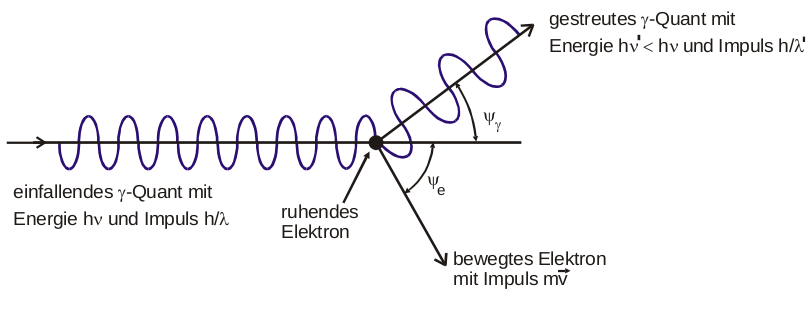
\includegraphics[height=5.5cm]{content/pictures/Compton.png}
   \caption{Compton-Streuprozesses als Schema dargestellt.\cite{V18}}
   \label{fig:Compton}
 \end{figure}

\subsubsection{Paarbildung}
Bei der Paarbildung wandelt sich das $\gamma$-Quant in ein Elektron und ein Positron um, falls es die dafür nötige Energie $E_{\gamma}>2m_{\symup{e}}c^2$ besitzt.
Damit dieser Prozess (vom Ruhesystem des $\gamma$-Quants aus gesehen) stattfinden kann, muss zusätzlich noch ein Stoßpartner vorhanden sein.
Ist dieser Partner ein Elektron, benötigt das $\gamma$-Quant aufgrund der Rückstoßenergie sogar die vierfache Ruhemasse des Elektrons an Energie, damit es zur Paarbildung kommen kann.
Der Wirkungsquerschnitt $\sigma_{\symup{Pa}}$ ist je nach Ort, an dem die Paarerzeugung stattfindet, unterschiedlich groß, da zum Beispiel im Bereich der K-Schale das gesamte Coulomb-Feld mitwirkt, bei äußeren Schalen
jedoch Abschirmungseffekte eine Rolle spielen, wodurch $\sigma_{\symup{Pa}}$ von der Abschirmung abhängt.
 \begin{figure}
   \centering
   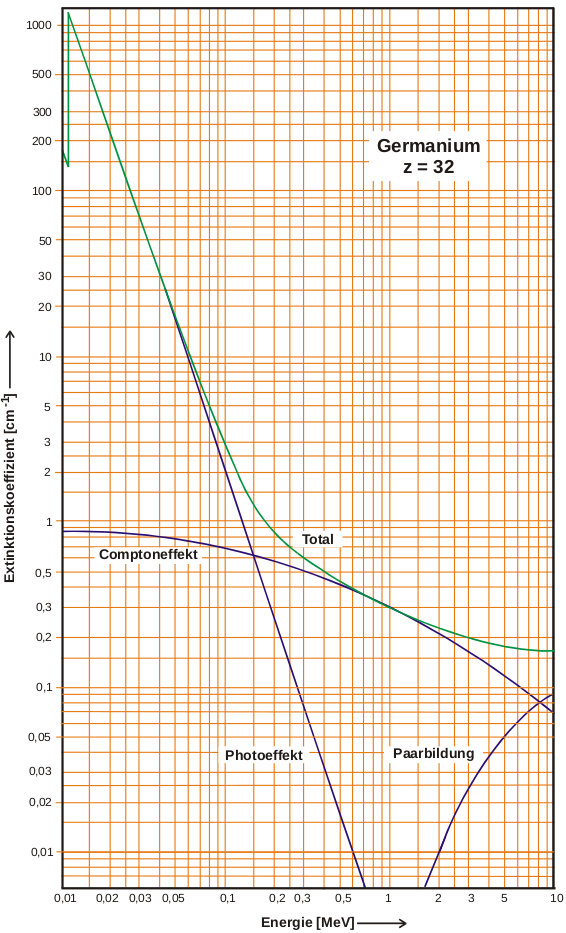
\includegraphics[height=23cm]{content/pictures/Germanium.png}
   \caption{Energieabhängigkeit des Extinktionskoeffizienten in Germanium.\cite{V18}}
   \label{fig:Germanium}
 \end{figure}

\subsection{Funktionsweise eines Reinst-Germanium-Detektors}
Der Reinst-Germanium-Detektor ist ein Halbleiter-Detektor, die Funktionsweise ähnelt also der einer Halbleiterdiode.
Folglich existieren im Materiel zwei aneinander grenzende unterschiedlich dotierte Schichten, die elektronenüberschüssige n-dotierte Schicht und die elektronenarme p-dotierte Schicht.
Die beweglichen Ladungsträger, die Elektronen und Löcher, nahe der Grenzfläche zwischen den dotierten Bereichen rekombinieren dort.
Der jetzige Mangel dieser beweglichen Ladungsträgern an der Grenzzone bildet eine ladungsträgerarme Zone oder Sperrschicht, die n-dotierte Seite der Sperrschicht ist positiv und die p-dotierte Seite negativ geladen.
Es entsteht ein inneres elektrisches Feld, was eine weitere Diffusion von Ladungsträgern verhindert.
Trifft ein $\gamma$-Quant auf diese ladungsträgerarme Zone, wird es durch die vorher genannten Effekte mit den Elektronen wechselwirken, die wiederum mit anderen Elektronen im Valenzband wechselwirken.
Die gestoßenen Elektronen gehen vom Valenzband zum Leitungsband über und hinterlassen Elektron-Loch-Paare.
Aufgrund des in der Sperrschicht erzeugtem elektrischen Feld werden die Löcher und Elektronen hinreichend schnell getrennt.
Werden diese Elektronen und Löcher, bevor sie wieder rekombinieren, an Elektroden gesammelt, wird ein Ladungsimpuls mit einem Betrag, der von der deponierten Energie des $\gamma$-Quants abhängig ist, gemessen.
Da die Absorptionswahrscheinlichkeit mit der Dicke exponentiell zunimmt (\ref{eq:Absorbtion}), wird eine äußere Spannung angelegt, wodurch die Sperrzone vergrößert wird.
Hier muss jedoch beachtet werden, dass durch thermische Effekte freie Ladungsträger in der Sperrzone vorhanden sind, die durch die Spannung getrennt und als Signale registriert werden.
Um diesen Störeffekt zu minimieren, wird der Detektor auf $\SI{77}{\kelvin}$ gekühlt.

Das Auflösungsvermögen ist eine wichtige Kenngröße eines Detektors.
Es wird durch die Halbwertsbreite $\Delta E_{\sfrac{1}{2}}$ der gemessenen Peaks bestimmt.
Der Detektor ist fähig zwei Spektrallinien mit Mittelwerten $E_1$ und $E_2$ zu unterschieden, wenn die Differenz mindestens $\Delta E_{\sfrac{1}{2}}$ beträgt (siehe Abb. \ref{fig:Breite}).
Die Breite der Linien hängt von der Zahl $n$ der erzeugten Elektron-Loch-Paare ab.
Der Mittelwert $\bar{n}$ entspricht dem Quotienten der Energie $E_{\gamma}$ der einfallenden $\gamma$-Quanten und der Bildungsenergie $E_{\symup{EL}}$ eines Elektron-Loch-Paares.
Weil Elektron-Loch-Paare nur durch Beteiligung von Phononen erzeugt werden können, ist die vom $\gamma$-Quant übertragene Energie auf den Detektor statistisch auf die Phononen- und Elektron-Loch-Paar Erzeugung verteilt.
Das hat zur Folge, dass der Fehler der (Poisson-) Verteilung durch einen Fano-Faktor $F$ korrigiert werden muss:
\begin{equation*}
\sigma = \sqrt{F\bar{n}}.
\end{equation*}
Bei Germanium beträgt $F$ etwa \num{0.1}.
Da $n$ sehr viel größer als \num{1} ist, kann die Poisson-Verteilung als Gauß-Verteilung approximiert werden.
Ist $\sigma_E$ die Standardabweichung, lässt sich die Halbwertsbreite aus
\begin{equation}
\label{eq:aufloesung}
\Delta E_{\sfrac{1}{2}} = 2 \cdot \sqrt{2\ln{(2)}}\cdot\frac{E_{\gamma}\sigma}{\bar{n}} \approx \num{2.35}\sqrt{\num{0.1} \cdot E_\gamma \cdot E_{\symup{El}}}
\end{equation}
errechnen.
Die Halbwertsbreite bei einem Germanium-Detektor mit einer typischen $\gamma$-Energie von $\SI{500}{\kilo\electronvolt}$ beträgt somit $\Delta E_{\sfrac{1}{2}} =\SI{895}{\electronvolt}$.
Zusätzliche Störeffekte sind Leckstrom des Halbleiterkristalls, Rauschen des Verstärkers (beide werden durch Kühlung minimiert) und Inhomogenitäten des elektrischen Feldes.

Unter der Vollenergienachweiseffizienz wird die Energieabhängigkeit der Nachweiswahrscheinlichkeit eines $\gamma$-Quants verstanden.
Nur $\gamma$-Quanten, die durch den Photoeffekt wechselwirken, deponieren ihre vollständige Energie im Detektor und sind für die Effizienz relevant.

 \begin{figure}
   \centering
   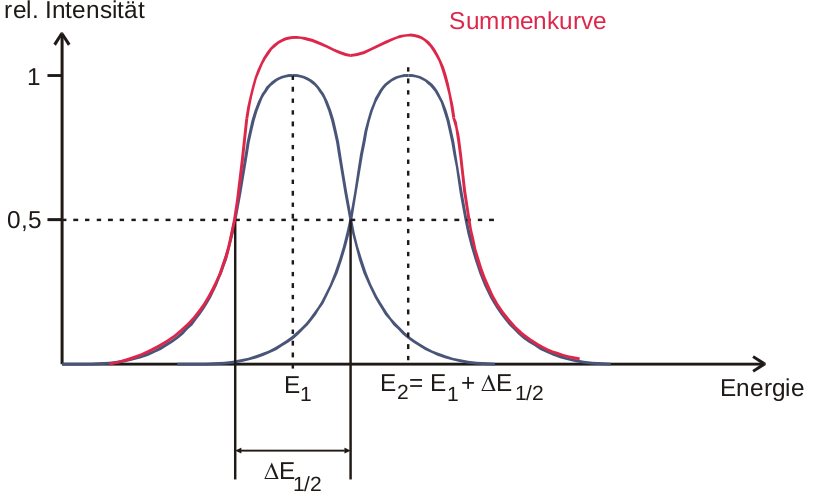
\includegraphics[height=7cm]{content/pictures/Breite.png}
   \caption{Die Halbwertsbreite als Maß des Auflösungsvermögens eines Detektors.\cite{V18}}
   \label{fig:Breite}
 \end{figure}

\subsection{Energiespektrum eines monochromatischen \texorpdfstring{$\gamma$}{gamma}-Strahlers}
Ein typisches Spektrum eines monochromatischen Strahlers ist in Abbildung \ref{fig:Spektrum} zu sehen.
Deutlich zu erkennen sind das Compton-Kontinuum mit der Compton-Kante und dem Rückstreupeak und der Vollenergiepeak.
Der Vollenergiepeak entsteht, wenn das $\gamma$-Quant durch den Photoeffekt und den Compton-Effekt seine vollständige Energie abgibt. 
Dieser Peak ist charakteristisch für sein aussendendes Nuklid.
Dessen Halbwertsbreite $\Delta E_{\sfrac{1}{2}}$ ist das ausschlaggebende Maß für das Auflösungsvermögen des Detektors.

Das Compton-Kontinuum reicht, durch die verschiedenen Streuwinkel der $\gamma$-Quanten, von der Energie \num{0} bis zur Compton-Kante $E_{\symup{e},\symup{max}}$ bei $\Psi{\gamma}=\SI{180}{\degree}$, mit
\begin{equation}
\label{eqn:Com_Kante}
E_{\symup{e},\symup{max}}=E_{\gamma}\frac{2\varepsilon}{1+2\varepsilon}.
\end{equation}
%und
%\begin{equation*}
%\epsilon = \frac{E_{\gamma}}{m_{\symup{e}} c^2}.
%\end{equation*}
Der Rückstreupeak entsteht durch $\gamma$-Quanten, die erst nach Compton-Streuung mit der Umgebung (Abschirmung des Detektors oder Quelle selbst) in den Detektor gelangen.
Dessen Energie ist
\begin{equation}
  \label{eqn:rueck}
  E_\text{Rück, theo} = \frac{1}{1+2\varepsilon} \cdot E_{\gamma}.
\end{equation}

Die dargestellte Empfindlichkeitsgrenze hat ihren Ursprung in der Wechselwirkung der $\gamma$-Quanten mit der Schutzhaube und der Oberfläche des Detektors.
Bei dem hier verwendeten Ge-Detektor liegt diese Grenze bei \SIrange{40}{50}{\kilo\electronvolt}.
 \begin{figure}
   \centering
   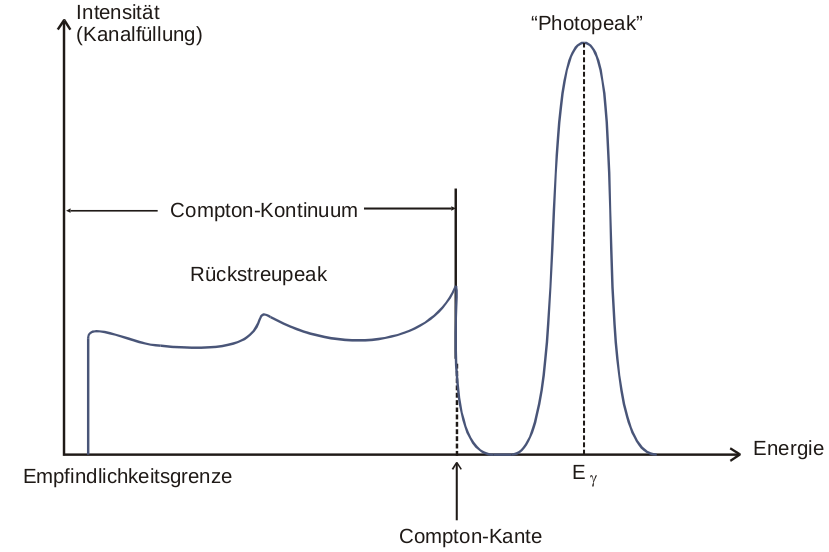
\includegraphics[height=9cm]{content/pictures/Spektrum.png}
   \caption{Typisches Spektrum eines monochromatischen Gammastrahlers.\cite{V18}}
   \label{fig:Spektrum}
 \end{figure}